\documentclass[10pt,twocolumn]{article}

\usepackage[a4paper,margin=0.66in,columnsep=0.24in]{geometry}
\usepackage{times}
\usepackage{graphicx}
\usepackage{booktabs}
\usepackage{wrapfig}
\usepackage{subcaption}
\usepackage{amsmath}
\usepackage{hyperref}
\usepackage{caption}
\usepackage{balance}

\captionsetup{font=small,labelfont=bf}
\setlength{\textfloatsep}{7pt plus 1pt minus 2pt}
\setlength{\floatsep}{7pt plus 1pt minus 2pt}
\setlength{\intextsep}{6pt plus 1pt minus 2pt}
\setlength{\abovecaptionskip}{3pt}
\setlength{\belowcaptionskip}{0pt}
\setlength{\parskip}{0pt}
\setlength{\parindent}{1em}

\title{\vspace{-0.38in}CIFAR-10 Classification with VGG-A Variants and Batch Normalization}
\author{\small Student Name: \textit{to be provided} \quad Student ID: \textit{to be provided}\\
\small Code: \href{https://github.com/yuheng-li-ai/deep_learning2}{GitHub repository} \quad
Dataset: \href{https://www.cs.toronto.edu/~kriz/cifar.html}{CIFAR-10 website} \quad
Trained weights: \href{https://www.modelscope.cn/models/yuhengli/deep-learning2-final-model/files}{ModelScope files}}
\date{}

\begin{document}
\maketitle
\vspace{-0.20in}

\begin{abstract}
This paper reports a controlled CIFAR-10 study of VGG-A-style convolutional networks, with emphasis on the role of Batch Normalization (BN) in both accuracy and optimization. The final selected model is a VGG-A-BN network with GELU activations, trained with Adam and cross-entropy loss, which reaches 83.96\% test accuracy and a 16.04\% test error. In the matched ReLU comparison, BN improves the VGG-A baseline from 76.51\% to 83.24\% best test accuracy while adding only 5,504 parameters. Optimization measurements further show that BN reduces the mean learning-rate loss-envelope width from 0.4084 to 0.2147 and lowers the maximum local gradient-difference-per-distance from 857.62 to 320.57 in the measured update directions. These results support BN as both a performance-improving architectural component and an optimization stabilizer for this CIFAR-10 setting.
\end{abstract}

\section{Introduction}
CIFAR-10 is a compact but nontrivial benchmark for studying the interaction between architecture, regularization, and optimization. The assignment requires a convolutional network containing fully connected layers, two-dimensional convolution, pooling, and nonlinear activations; it also requires controlled trials over capacity, loss or regularization, activation functions, optimizers, and model-inspection visualizations. I use VGG-A as the central architecture because it satisfies the required components while remaining transparent enough for matched ablations.

The main question is not merely which run obtains the lowest test error. Batch Normalization is explicitly part of the project, and the report therefore examines whether BN changes training behavior in ways that are visible beyond a final accuracy number. The evidence is organized around three levels: ordinary classification performance, sensitivity to learning-rate choices through a loss envelope, and a local gradient-smoothness measurement motivated by first-order optimization.

\section{Method}
\subsection{Data and Training Protocol}
All experiments use the standard CIFAR-10 training split for optimization and the standard test split for reporting. Images are converted to tensors and normalized with channel-wise mean $(0.5,0.5,0.5)$ and standard deviation $(0.5,0.5,0.5)$. Unless stated otherwise, training uses 20 epochs, batch size 128, random seed 2020, Adam with learning rate $10^{-3}$, zero weight decay, and cross-entropy loss. The reported test accuracy is the best accuracy observed during the 20 epochs, and test error is computed as $1-\mathrm{accuracy}$.

\subsection{Model Family}
\begin{wrapfigure}{r}{0.40\columnwidth}
  \vspace{-0.15in}
  \centering
  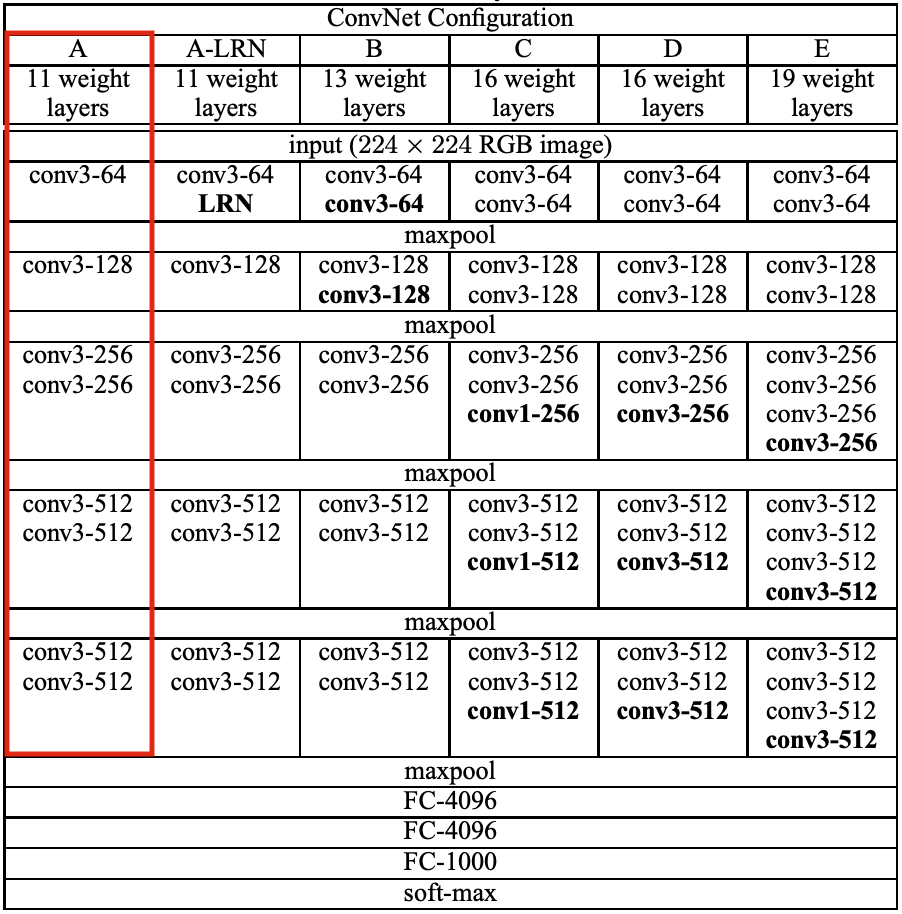
\includegraphics[width=0.39\columnwidth]{pic/vgg.png}
  \caption{VGG-style feature extractor used as the baseline design.}
  \label{fig:vgg}
  \vspace{-0.16in}
\end{wrapfigure}
The baseline is a VGG-A network adapted to $32\times32$ input images. It contains five convolutional stages, max pooling between stages, ReLU nonlinearities, and a three-layer classifier with two hidden fully connected layers of width 512. The BN variant inserts \texttt{BatchNorm2d} after each convolution and before the activation. Additional runs vary classifier dropout, network width, optimizer, activation, and label smoothing. This design gives direct evidence for the architectural and optimization requirements without relying on an off-the-shelf public model.

\section{Classification Results}
Table~\ref{tab:main} summarizes the principal experiments. The plain VGG-A baseline reaches 76.51\% best test accuracy, while the matched VGG-A-BN run reaches 83.24\%. The difference is substantial because all other training settings are held fixed. BN also reaches its best epoch earlier, at epoch 12 rather than epoch 18, which suggests faster useful convergence rather than a late accidental improvement. The final selected architecture adds GELU activations on top of BN and reaches 83.96\% best accuracy, corresponding to a 16.04\% best test error.

\begin{table*}[t]
\centering
\caption{Main CIFAR-10 results. All runs use 20 epochs and batch size 128.}
\label{tab:main}
\small
\begin{tabular}{lrrrrrr}
\toprule
Model & Optimizer & Params & Best Acc. & Best Err. & Best Epoch & Final Acc.\\
\midrule
VGG-A & Adam & 9,750,922 & 0.7651 & 0.2349 & 18 & 0.7411\\
VGG-A-BN & Adam & 9,756,426 & 0.8324 & 0.1676 & 12 & 0.8257\\
VGG-A-Dropout & Adam & 9,750,922 & 0.7419 & 0.2581 & 12 & 0.7348\\
VGG-A-Light & Adam & 285,162 & 0.7027 & 0.2973 & 9 & 0.6818\\
VGG-A-BN & AdamW & 9,756,426 & 0.8302 & 0.1698 & 20 & 0.8302\\
VGG-A-BN-LeakyReLU & Adam & 9,756,426 & 0.8254 & 0.1746 & 18 & 0.8194\\
VGG-A-BN-GELU & Adam & 9,756,426 & \textbf{0.8396} & \textbf{0.1604} & 19 & \textbf{0.8373}\\
VGG-A-BN-GELU-LS & Adam & 9,756,426 & 0.8374 & 0.1626 & 19 & 0.8170\\
\bottomrule
\end{tabular}
\end{table*}

\begin{figure*}[t]
  \centering
  \begin{subfigure}{0.49\textwidth}
    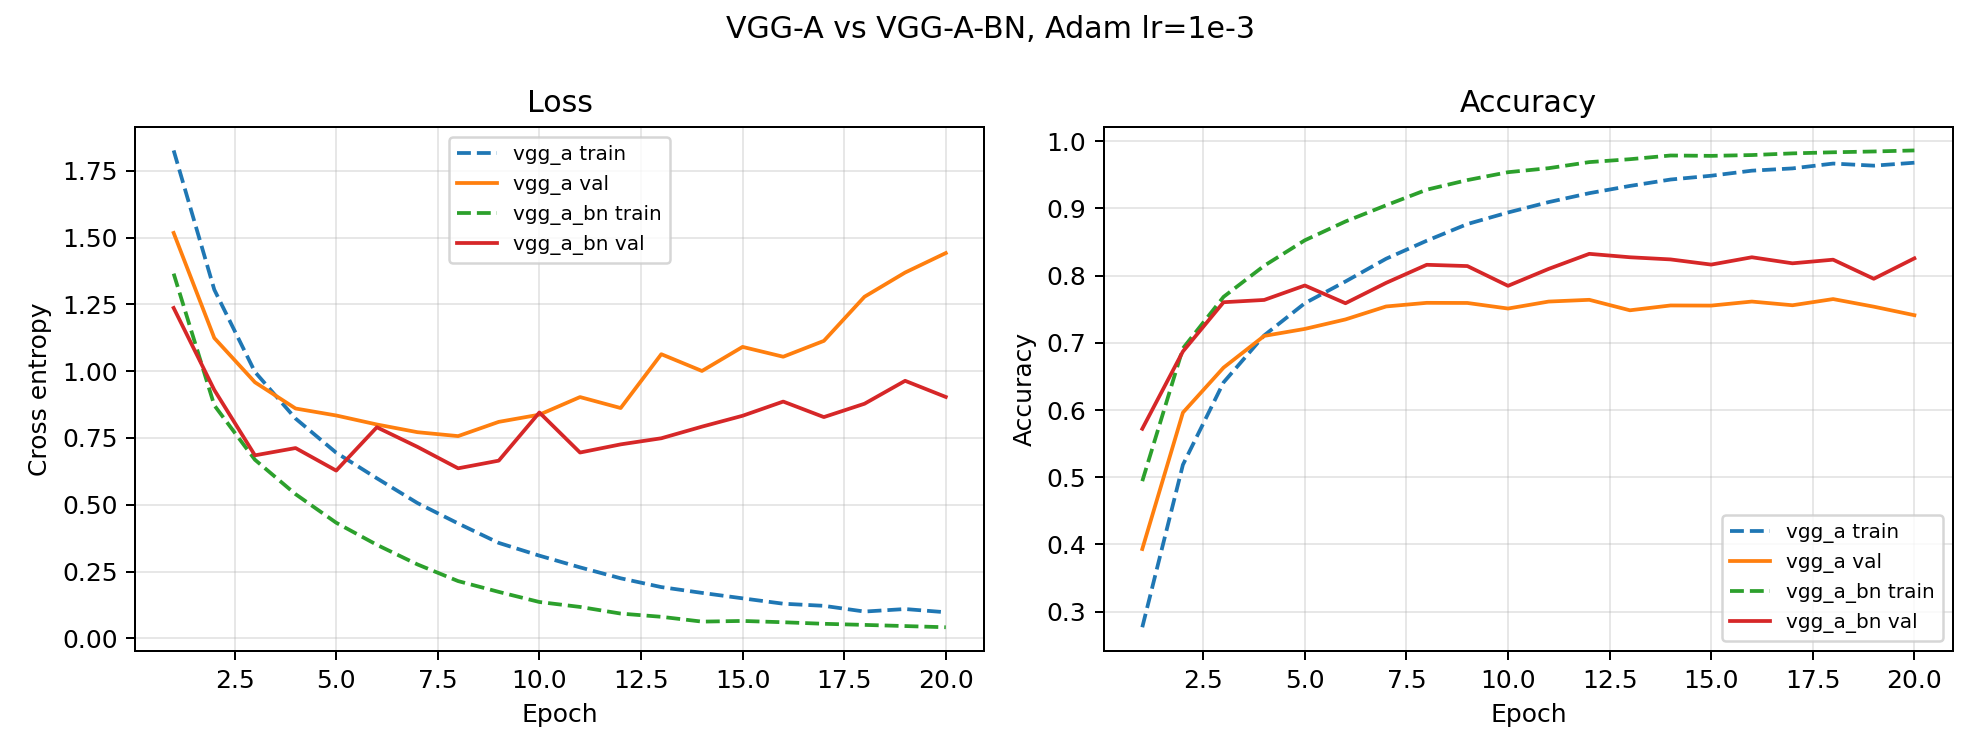
\includegraphics[width=\linewidth]{reports/figures/vgg_a_vs_bn_adam_lr1e-3.png}
    \caption{Matched VGG-A and VGG-A-BN runs.}
  \end{subfigure}
  \hfill
  \begin{subfigure}{0.49\textwidth}
    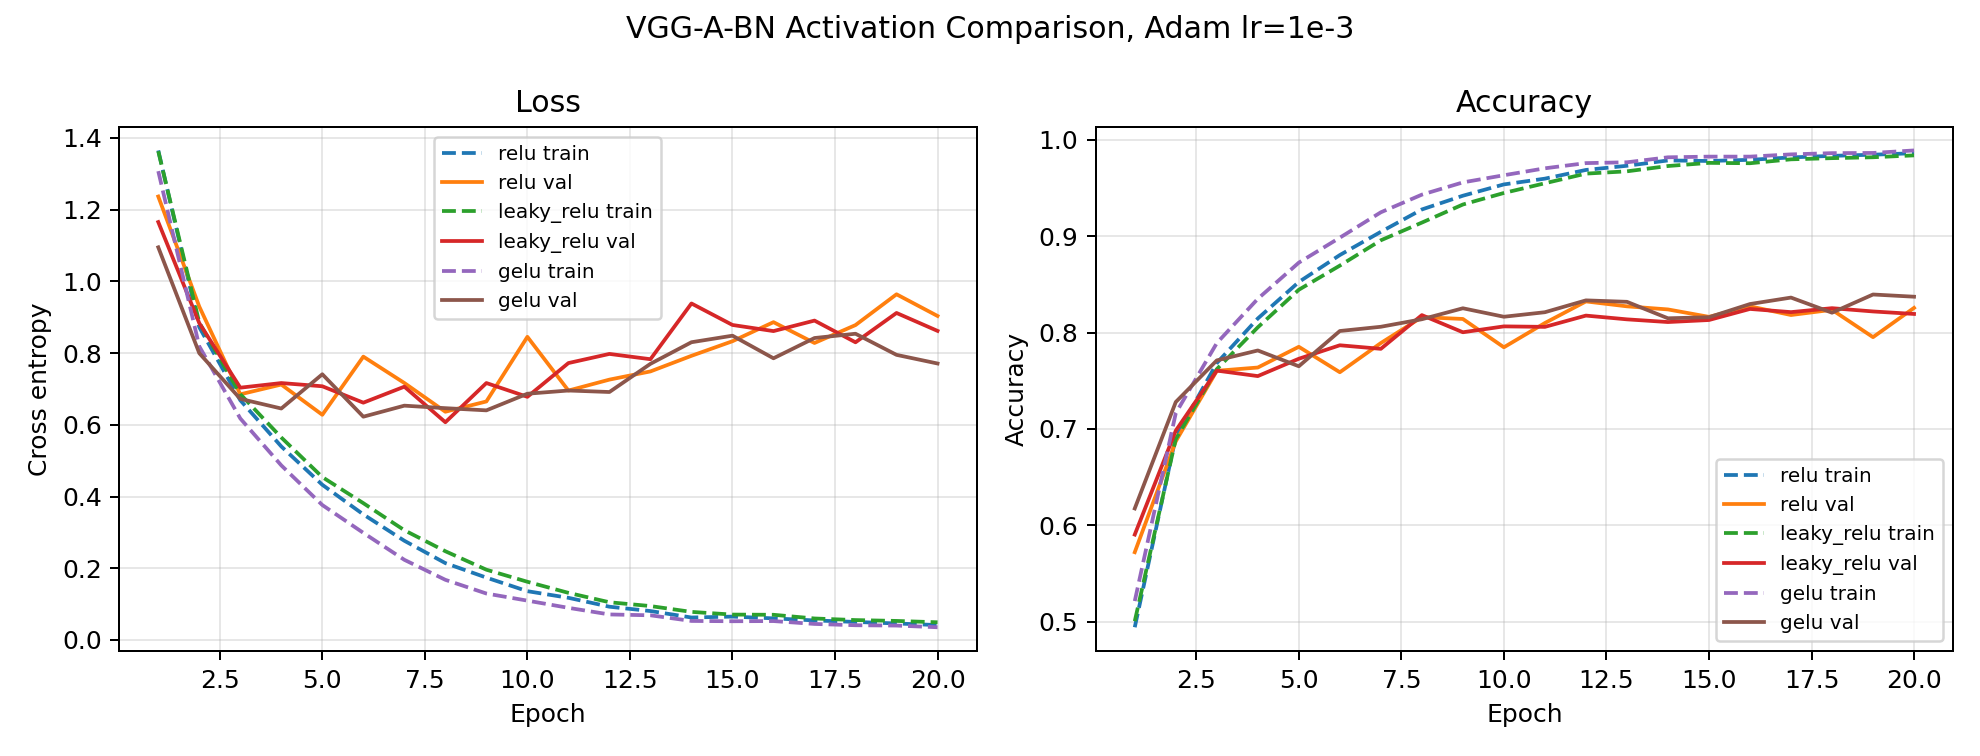
\includegraphics[width=\linewidth]{reports/figures/vgg_a_bn_activation_comparison_adam_lr1e-3.png}
    \caption{Activation functions on VGG-A-BN.}
  \end{subfigure}
  \caption{Training curves for the central BN comparison and the activation ablation.}
  \label{fig:main-curves}
\end{figure*}

The curves in Fig.~\ref{fig:main-curves} clarify the table. In the matched comparison, the BN model enters a higher test-accuracy regime much earlier than the plain baseline and remains there. The baseline ultimately obtains high training accuracy, but its final test loss is 1.4421, much larger than the BN model's 0.9035. The activation ablation shows that GELU is the strongest tested nonlinearity in this architecture. LeakyReLU does not improve peak accuracy over ReLU, whereas GELU improves both peak and final test accuracy.

Capacity and regularization ablations are informative but do not change the final model choice. VGG-A-Light reduces the parameter count to 285,162, only 2.92\% of the full model, but loses too much accuracy. Classifier dropout reaches only 74.19\% best accuracy, lower than the plain baseline. Label smoothing with smoothing factor 0.1 reaches a similar peak to the plain GELU model, 83.74\%, but finishes worse at 81.70\%; it is therefore useful as a required loss-regularization ablation rather than as the final submission model.

\section{Batch Normalization and Optimization}
\subsection{Learning-Rate Loss Envelope}
The assignment asks how BN helps optimization, so I trained VGG-A and VGG-A-BN with four learning rates: $10^{-4}$, $5\times10^{-4}$, $10^{-3}$, and $2\times10^{-3}$. For every update step, the training loss was saved. For each model family and step index, I computed the minimum and maximum loss across the four learning-rate runs and filled the region between these two curves. This measures how dispersed the loss trajectories are under different step-size choices.

\begin{wrapfigure}{r}{0.58\columnwidth}
  \vspace{-0.13in}
  \centering
  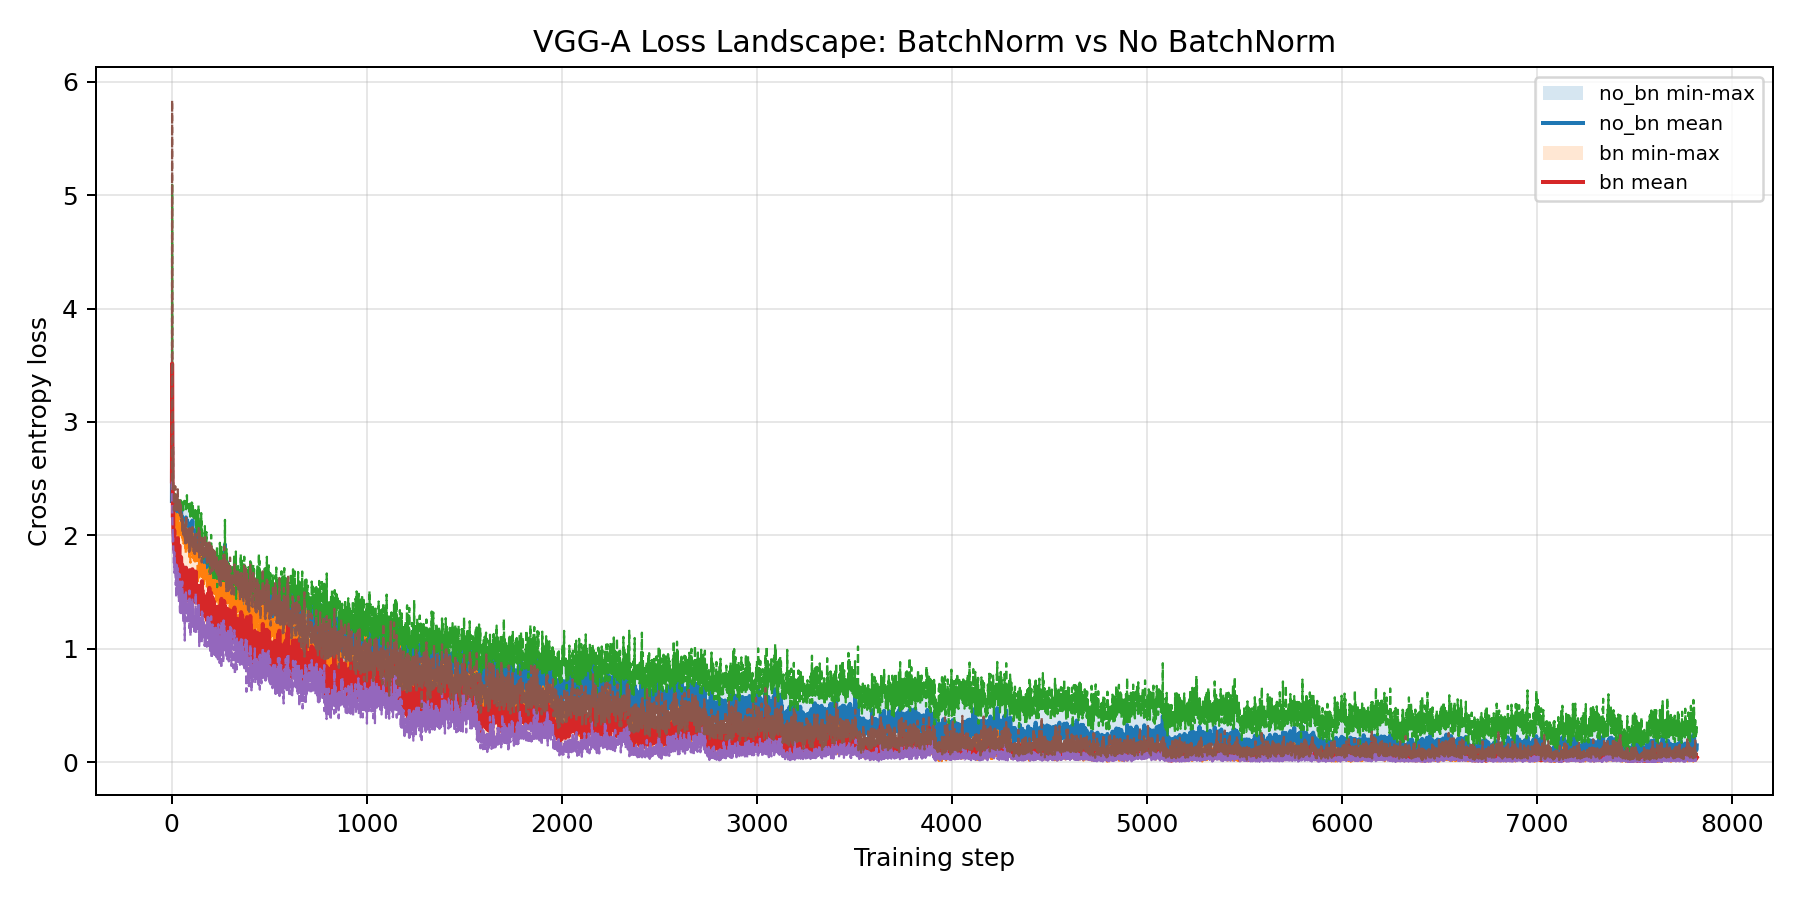
\includegraphics[width=0.57\columnwidth]{reports/figures/vgg_a_loss_landscape_bn_vs_no_bn.png}
  \caption{Per-step loss envelopes across four learning rates.}
  \label{fig:envelope}
  \vspace{-0.15in}
\end{wrapfigure}
The result in Fig.~\ref{fig:envelope} shows a narrower average envelope for BN. The no-BN mean envelope width is 0.4084, while the BN mean envelope width is 0.2147, a 47.4\% reduction. The final loss range is also much smaller with BN: 0.0306--0.0551 rather than 0.0576--0.2764. The maximum instantaneous width is larger for BN, 3.5587 versus 2.7904, because the $10^{-4}$ BN run converges slowly while the larger learning rates improve rapidly. This transient does not overturn the average and final-envelope evidence, which indicates lower sensitivity to the tested learning-rate choices.

\subsection{Gradient Predictiveness}
The loss envelope measures trajectory dispersion but does not directly measure the local linear approximation used by first-order optimization. I therefore added a separate local analysis around the trained VGG-A and VGG-A-BN checkpoints. For a validation subset of 512 examples, I computed the loss $L(w)$ and gradient $\nabla L(w)$, then evaluated points $w' = w-\eta\nabla L(w)$ for $\eta\in\{10^{-4},5\times10^{-4},10^{-3},2\times10^{-3}\}$. The first-order prediction error is
\[
\left|L(w')-\left(L(w)-\eta\|\nabla L(w)\|^2\right)\right|,
\]
and the gradient-difference-per-distance is
\[
\frac{\|\nabla L(w')-\nabla L(w)\|}{\|w'-w\|}.
\]

\begin{figure}[t]
  \centering
  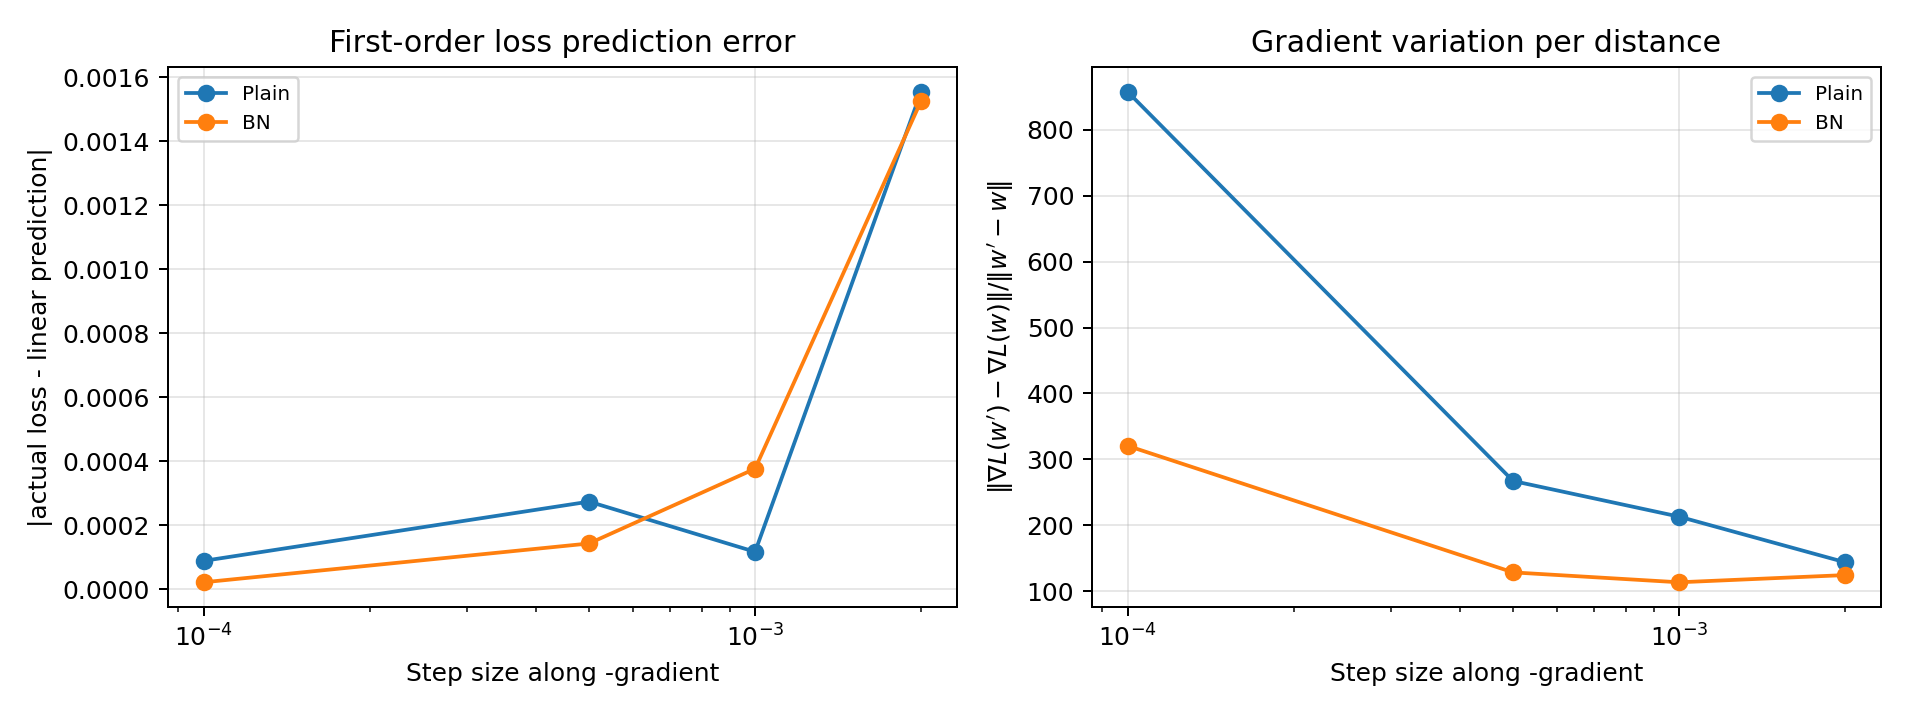
\includegraphics[width=\columnwidth]{reports/figures/vgg_a_gradient_smoothness_bn_vs_no_bn.png}
  \caption{Local first-order prediction error and gradient variation around trained VGG-A and VGG-A-BN checkpoints.}
  \label{fig:grad}
\end{figure}

Figure~\ref{fig:grad} gives a more nuanced picture than a single accuracy table. The mean prediction errors are almost identical, 0.0005088 for the plain checkpoint and 0.0005172 for BN, so this particular local measurement does not justify claiming a large BN advantage in loss predictiveness. The gradient-difference-per-distance is different: the maximum value falls from 857.62 for the plain checkpoint to 320.57 for the BN checkpoint. This supports the more specific conclusion that, along the tested update directions, the BN checkpoint has less abrupt gradient variation.

\section{Discussion}
The experiments indicate that BN is the most important tested modification to VGG-A. It improves accuracy, improves convergence speed, and makes the training loss less dispersed across the learning-rate choices used in the landscape experiment. GELU then gives a smaller but measurable gain on top of BN. AdamW gives a slightly better final state than Adam for the ReLU BN model, but not a better peak within 20 epochs. The label-smoothing run is also instructive: it nearly matches the best GELU peak accuracy but does not maintain the final accuracy, which suggests that this regularization choice is not automatically beneficial under the fixed schedule.

The optimization results should be interpreted carefully. A narrower learning-rate envelope does not prove a globally flatter Hessian landscape. The 3D surface in the appendix is also only a random two-dimensional slice. The stronger claims are therefore local and empirical: BN reduces the dispersion of loss trajectories across the tested step sizes, and it reduces the measured maximum gradient-difference-per-distance around the trained checkpoint. These observations are consistent with the view that BN makes the optimization process easier to control.

\section{Conclusion}
The final selected model is VGG-A-BN-GELU trained with Adam and plain cross-entropy loss. It reaches 83.96\% test accuracy and a 16.04\% test error on CIFAR-10. The project requirements are satisfied by a network containing convolution, pooling, activation, and fully connected layers; by ablations over width, dropout, label smoothing, activations, and optimizers; and by visualizations of training curves, loss envelopes, gradient smoothness, and local loss surfaces. The main finding is that BN provides the largest improvement in this study, raising matched VGG-A accuracy by 6.73 percentage points while also stabilizing optimization measurements.

\balance
\begin{thebibliography}{9}
\bibitem{cifar10}
A. Krizhevsky and G. Hinton, ``Learning multiple layers of features from tiny images,'' 2009.

\bibitem{pytorch}
PyTorch, ``Training a classifier,'' CIFAR-10 tutorial, \href{https://pytorch.org/tutorials/beginner/blitz/cifar10_tutorial.html}{online}.

\bibitem{bn}
S. Ioffe and C. Szegedy, ``Batch Normalization: Accelerating deep network training by reducing internal covariate shift,'' ICML, 2015.

\bibitem{bnopt}
S. Santurkar, D. Tsipras, A. Ilyas, and A. Madry, ``How Does Batch Normalization Help Optimization?'' NeurIPS, 2018.

\bibitem{adam}
D. P. Kingma and J. Ba, ``Adam: A method for stochastic optimization,'' arXiv:1412.6980, 2014.

\bibitem{vgg}
K. Simonyan and A. Zisserman, ``Very deep convolutional networks for large-scale image recognition,'' ICLR, 2015.
\end{thebibliography}

\appendix
\section{Appendix: Additional Experimental Details}
\subsection{Learning-Rate Sweep}
Table~\ref{tab:lr} lists the eight learning-rate sweep runs used for the loss-envelope plot. The BN model is weak at $10^{-4}$ under the 20-epoch budget, but it is strong and stable for $5\times10^{-4}$, $10^{-3}$, and $2\times10^{-3}$.

\begin{center}
\centering
\captionof{table}{Learning-rate sweep for VGG-A and VGG-A-BN.}
\label{tab:lr}
\scriptsize
\begin{tabular}{llrrr}
\toprule
Model & LR & Best Acc. & Final Acc. & Final Loss\\
\midrule
VGG-A & $10^{-4}$ & 0.7659 & 0.7526 & 1.3084\\
VGG-A & $5{\times}10^{-4}$ & 0.7840 & 0.7801 & 1.2380\\
VGG-A & $10^{-3}$ & 0.7651 & 0.7411 & 1.4421\\
VGG-A & $2{\times}10^{-3}$ & 0.7289 & 0.7179 & 1.1336\\
VGG-A-BN & $10^{-4}$ & 0.7453 & 0.7203 & 1.6119\\
VGG-A-BN & $5{\times}10^{-4}$ & 0.8244 & 0.8244 & 0.8311\\
VGG-A-BN & $10^{-3}$ & 0.8324 & 0.8257 & 0.9035\\
VGG-A-BN & $2{\times}10^{-3}$ & 0.8305 & 0.8192 & 0.8693\\
\bottomrule
\end{tabular}
\end{center}

\subsection{Loss Regularization}
\begin{center}
  \centering
  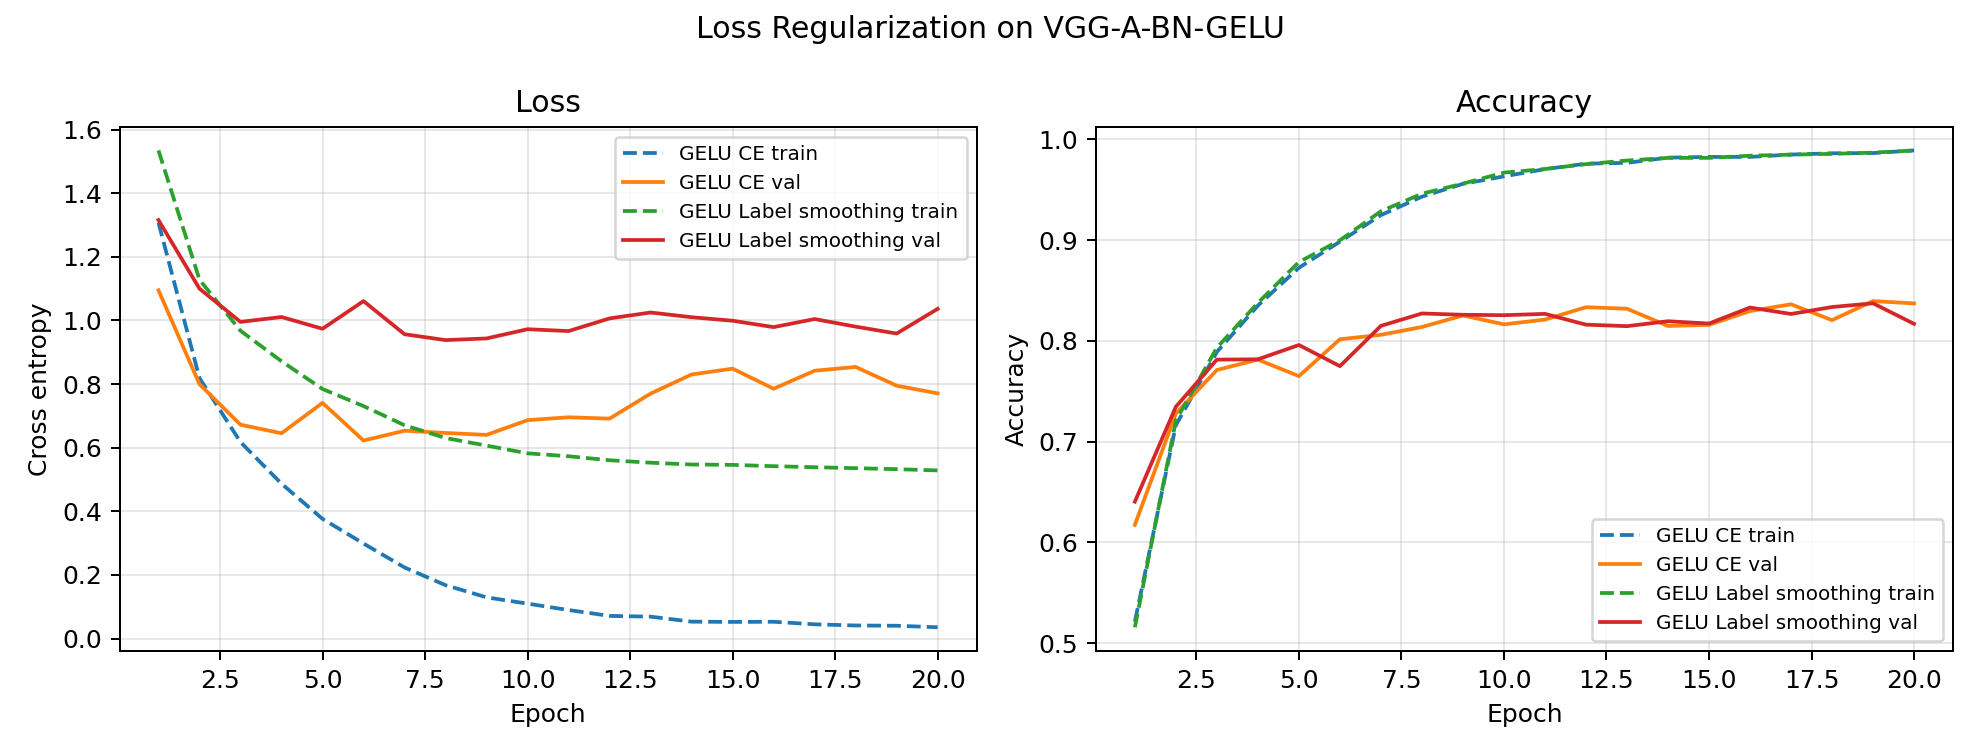
\includegraphics[width=\columnwidth]{reports/figures/vgg_a_bn_gelu_label_smoothing_comparison.png}
  \captionof{figure}{Plain cross entropy and label smoothing on the final VGG-A-BN-GELU architecture.}
  \label{fig:labelsmoothing}
\end{center}
Figure~\ref{fig:labelsmoothing} compares the final model under ordinary cross entropy and cross entropy with label smoothing 0.1. The smoothed run reaches 83.74\% best accuracy, close to the plain run's 83.96\%, but its final accuracy is lower. This run is retained as evidence for the loss-function and regularization requirement, not as the selected model.

\subsection{Local 3D Surface}
\begin{center}
  \centering
  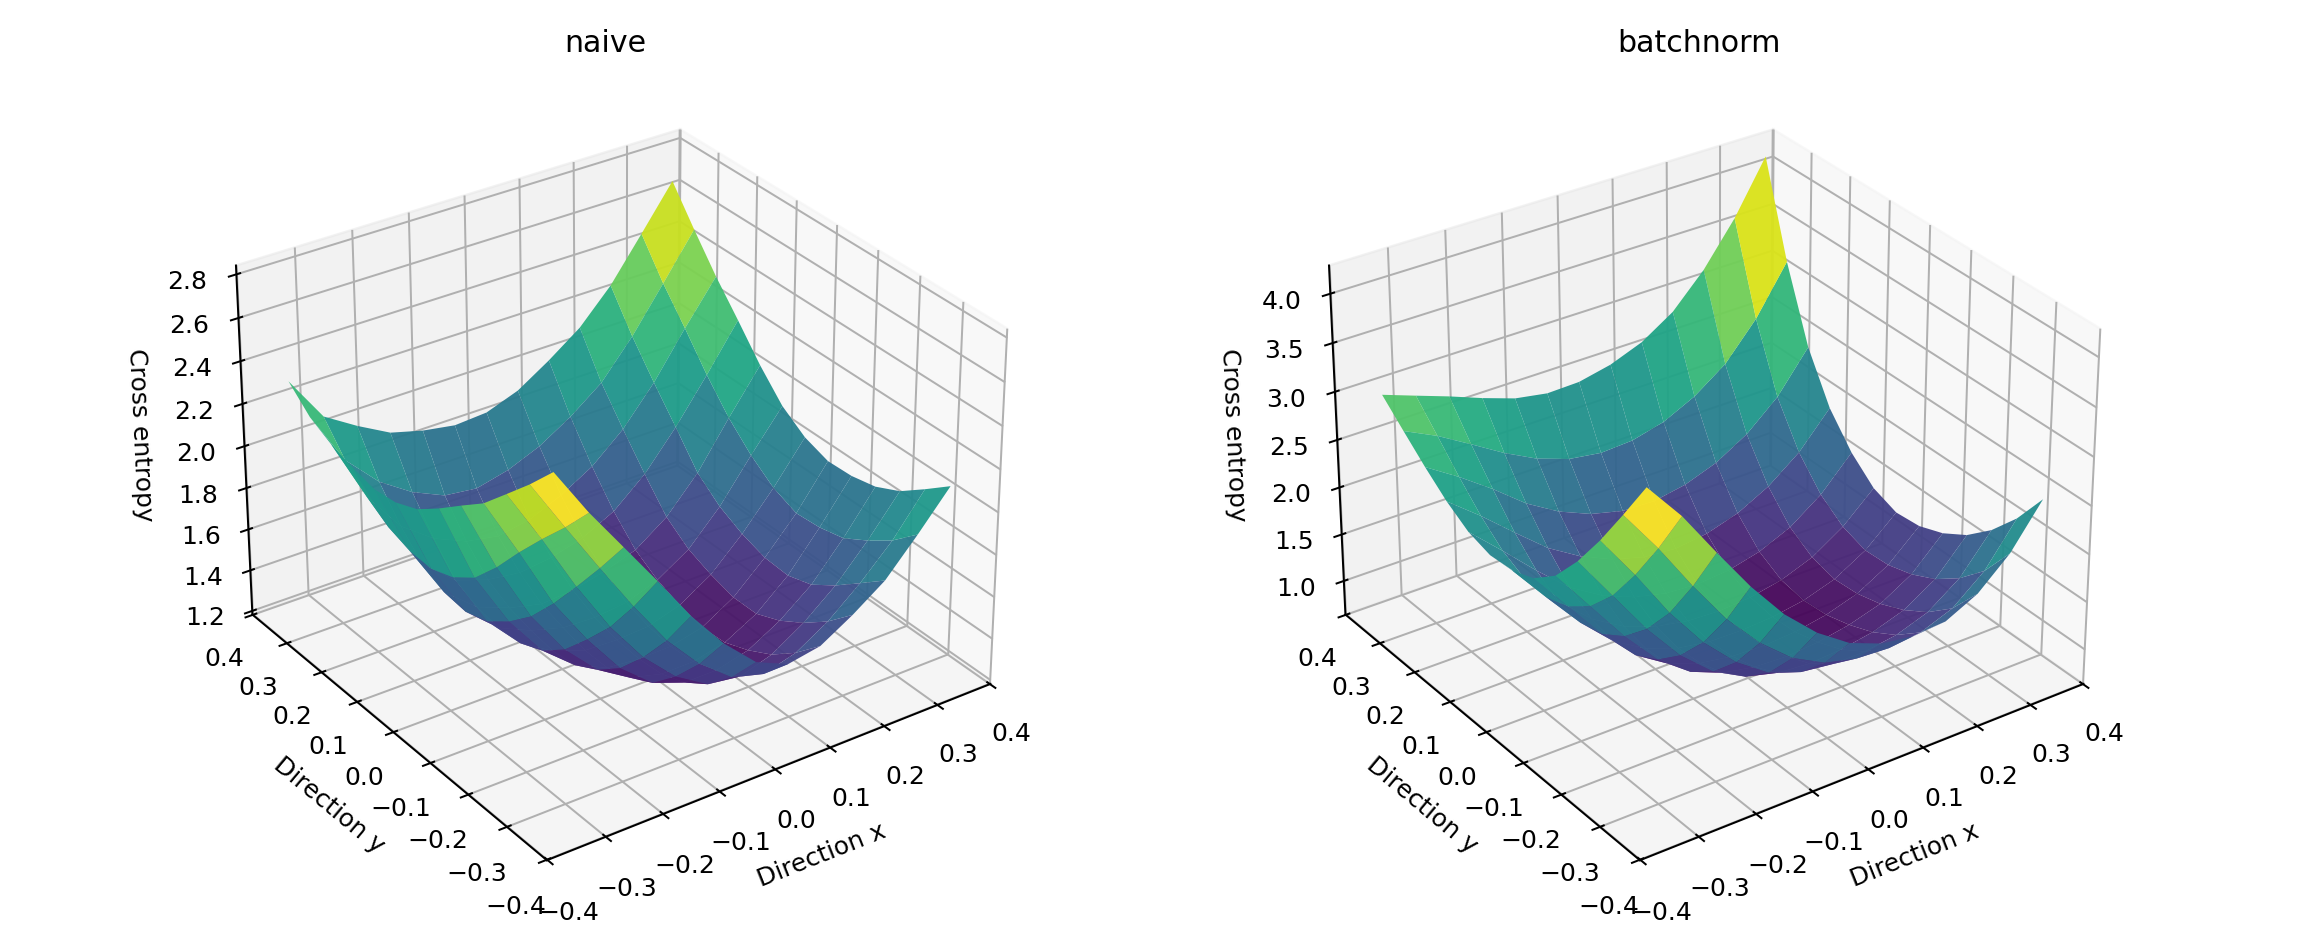
\includegraphics[width=\columnwidth]{reports/figures/vgg_a_3d_loss_surface_naive_vs_bn.png}
  \captionof{figure}{Random two-dimensional loss-surface slices around trained VGG-A and VGG-A-BN checkpoints.}
  \label{fig:surface3d}
\end{center}
The 3D surface visualization in Fig.~\ref{fig:surface3d} uses two random normalized parameter-space directions, a $13\times13$ grid with radius 0.35, and 1,024 validation examples. The center loss is 1.2258 for VGG-A and 0.7133 for VGG-A-BN. Because random two-dimensional slices depend on direction choice, this figure is treated as qualitative support rather than the primary smoothness metric.

\subsection{Requirement Coverage}
The code includes the required network components: convolutional layers, max-pooling layers, activation functions, and fully connected layers. It also includes optional components through BN and dropout. Different width settings are represented by VGG-A and VGG-A-Light, different activations by ReLU, LeakyReLU, and GELU, different optimizers by Adam and AdamW, and different loss regularization by plain cross entropy versus label smoothing. All formal outputs are written to separate run directories, and the training script now refuses accidental overwrites unless explicitly instructed.

\end{document}
